\documentclass{article}

\usepackage[utf8]{inputenc}
\usepackage[T1]{fontenc}
\usepackage[francais]{babel}
\usepackage{titling}
\setlength{\droptitle}{-3cm}
\usepackage{graphicx}
\usepackage{underscore}
\usepackage{hyperref} 


\title{Description des choix : outils/logiciels et modélisation}
\author{CAROT Axel, ARISOY Ivan Can, \\ DARDE Guilhem, NDJINGA NDJINGA Anta Claude}
\date{\today}

\begin{document}
\maketitle

\section{Choix des Outils et Logiciels pour le Projet}
\subsection{Utilisation des Notebooks Kaggle}
Dans le cadre de notre projet, nous avons opté pour des notebooks Kaggle car ils fournissent un accès gratuit aux ressources GPU. L'utilisation de GPU est cruciale pour l'entraînement efficace de nos modèles d'apprentissage en permettant une réduction significative des temps d'entraînement.

\begin{figure}[h]
    \centering
    
\includegraphics[width=0.4\textwidth]{kaggle.png}
    \caption{logo kaggle}
    \label{fig:kaggle}
\end{figure}

Concernant le stockage et l'accessibilité des données, Kaggle offre un espace de stockage pratique et facilement accessible pour toute l'équipe. De plus, les notebooks Kaggle  nous permettent de collaborer et facilite donc le travail d'équipe en permettant à plusieurs utilisateurs de contribuer simultanément au même projet. 

\subsection{Le Choix du Langage Python}

Le langage Python s'est naturellement imposé comme le langage de programmation pour notre projet, car nous sommes plus à l'aise avec ce langage, et certains d'entre nous l'utilisent dans leur formation en alternance. \\

Python propose de nombreuses bibliothèques telles que Numpy et Pandas, qui sont indispensables pour la manipulation efficace des données. Matplotlib et Seaborn nous ont permis de réaliser des visualisations dans le cadre de nos analyses descriptives. \\

Pour l'apprentissage automatique, nous utilisons Scipy et Sklearn, qui offrent une gamme d'outils pour le prétraitement des données, l'analyse statistique et la mise en œuvre d'algorithmes d'apprentissage. Nous faisons également appel à des bibliothèques comme Torch (PyTorch), Transformers et Spacy pour l'apprentissage et le traitement du langage naturel. \\

Des outils tels que Numba et GPUtil maximisent l'efficacité de notre code en optimisant les performances et en gérant efficacement les ressources matérielles, notamment les GPU.

\subsection{Approche collaborative}
\subsubsection{Collaboration dans le groupe}
Nous disposons d'un dépôt privé sur GitHub, qui est utilisé pour la gestion collaborative du code et qui nous permet de suivre toutes les modifications apportées à notre code et à nos rapports. Ce dépôt inclut un fichier README pour une présentation concise du projet, ainsi que divers dossiers organisant notre travail, comme les comptes-rendus de réunions, les données, les notebooks et les rapports. \\

Pour la rédaction collaborative de nos rapports, nous utilisons Overleaf, qui permet à tous les membres de l'équipe de travailler simultanément sur les mêmes documents. \\

Nous avons également créé un serveur Discord pour la communication et la gestion du projet. Ce serveur est structuré en plusieurs chaînes, chacune étant dédiée à un aspect spécifique de notre collaboration : discussions générales, planification des sessions de travail, partage de ressources bibliographiques et suivi des échéances. \\

Trello nous aide à visualiser et à suivre la progression des différentes tâches du projet. Chaque tâche est attribuée à un membre de l'équipe et associée à une date limite.

\subsubsection{Reproductibilité, collaboration externe}
Les notebooks Kaggle, ainsi que les diverses bibliothèques Python que nous utilisons, sont compatibles avec différents systèmes d'exploitation, fonctionnant sans problème sur les principaux OS tels que Windows, macOS et Linux. Cette flexibilité garantit que tous les membres de l'équipe peuvent travailler efficacement, quel que soit leur système d'exploitation. \\

Concernant la reproductibilité de notre approche, nous avons ajouté des commentaires pour expliquer le code, les méthodes utilisées et les étapes des processus effectués. De plus, toute personne souhaitant reproduire notre approche et à qui nous aurions autorisé l'accès à nos notebooks aurait également accès aux données stockées sur Kaggle, ce qui assure une bonne reproductibilité de nos processus.

\section{Choix des modélisations pour le Projet}

Le pipeline pour l'analyse spatio-temporelle des données textuelles établi par nos commanditaires comporte les étapes principales suivantes :
\begin{itemize}
    \item Acquisition des données
    \item Traitement du texte
    \item La sélection d'articles pertinents comportant des termes clés spécifiques (word embedding)
    \item Modélisation de sujets (LDA)
    \item Développement de l'indicateur TXT-FS
    \item L'application et la mise en œuvre concrète des données traitées. \\
\end{itemize}

Nos commanditaires ont exprimé le désir d'apporter des améliorations au pipeline existant qui utilise une modélisation simple. Nous avons décidé, en conséquence, de remplacer les techniques de sélection d'articles pertinents (word embedding) et de modélisation de sujets (LDA) par des modèles plus complexes tels que BERT (modèle de langage de grande envergure), CamemBERT, et le filtrage de pertinence inspiré de FlauBERT.
\begin{figure}[h]
    \centering
    
\includegraphics[width=0.5\textwidth]{BERT.png}
    \caption{logo CamemBERT}
    \label{fig:CamemBERT}
\end{figure}

Les conditions d’application de ces méthodes sont respectées puisque nous disposons de données textuelles en grande quantité (corpus comportant plus de 20 000 articles). Les articles sont longs et variés ce qui permet capturer efficacement le contexte linguistique. Nos données sont diversifiées, abondantes et représentatives de la langue et des sujets spécifiques à notre étude. Cela permet de réduire le risque de potentitiels biais significatifs qui pourraient fausser les modélisations.

\subsection{Modèle de classification}
\subsubsection{Classification manuelle des articles pertinents pour le jeu d'entraînement}
Pour entraîner notre modèle de classification, nous avons tout d'abord classifié manuellement un échantillon d'articles comme étant pertinents ou non. Pour ce faire, nous avons établi les critères essentiels permettant de déterminer la pertinence d'un article :
\begin{itemize}
    \item Identifier les articles qui traitent directement de thèmes liés à la sécurité alimentaire, comme l'agriculture, la pêche, l'élevage, les cultures vivrières, les politiques alimentaires, les programmes d'aide alimentaire, etc.
    \item Identifier des mots-clés et des termes spécifiques à la sécurité alimentaire définis dans des lexiques français qui nous ont été fournis et qui ont été élaborés par nos commanditaires ainsi que plusieurs experts en sécurité alimentaire.    
    \item Se concentrer sur les articles qui mentionnent spécifiquement des pays ou des régions d'Afrique de l'Ouest. \\
\end{itemize}

La classification manuelle des articles est cruciale pour l'entraînement d'un modèle de classification supervisé, car elle fournit des données étiquetées précises, servant de référence au modèle pour apprendre à distinguer les articles pertinents et non pertinents. En établissant des critères clairs et en classifiant manuellement un échantillon d'articles, on crée un ensemble de données d'entraînement fiable qui guide le modèle à reconnaître les caractéristiques spécifiques associées à la pertinence. Cette classification incorpore des connaissances métier spécialisées grâce à l'utilisation des lexiques, ce qui participe à la fiabilité des données d'entraînement.

\subsubsection{Sélection et configuration du modèle}
Nous avons choisi \texttt{CamembertForSequenceClassification} car il a été spécialement pré-entraîné sur un vaste corpus français, ce qui est très important pour bien classer les articles sur la sécurité alimentaire. Ce modèle a appris à partir d'une grande quantité de textes en français et a été ensuite entraîné avec nos articles que nous avons classifiés manuellement. \\

Le modèle \textbf{CamembertModèle} est une base pour traiter les textes, mais il n'est pas utilisable tel quel pour classer les articles dans des catégories précises. Nous aurions dû lui ajouter des éléments supplémentaires. Par contre, \texttt{CamembertForSequenceClassification} est déjà équipé pour cette tâche. Il est conçu spécialement pour classer des textes complets dans des catégories. Dans notre cas, article pertinent pour la sécurité alimentaire ou non. Ce modèle nous aide à comprendre le sens global des articles et à les classer correctement selon nos besoins.

\subsection{Hyperparamètres et optimisation}
\subsubsection{L'optimiseur AdamW}
L'optimiseur AdamW est une extension de l'optimiseur Adam qui inclut la perte de poids pour la régularisation. C'est un outil utilisé pour ajuster et améliorer notre modèle pendant son entraînement. Il ajuste automatiquement le taux d'apprentissage en fonction de l'estimation des premier et deuxième moments des gradients, ce qui le rend plus efficace pour les modèles complexes tels que les transformateurs. En somme, il aide à éviter certains problèmes communs en ajustant lui-même à quel point il change le modèle à chaque étape de l'apprentissage. \cite{adamw}.

\begin{figure}[h]
    \centering
    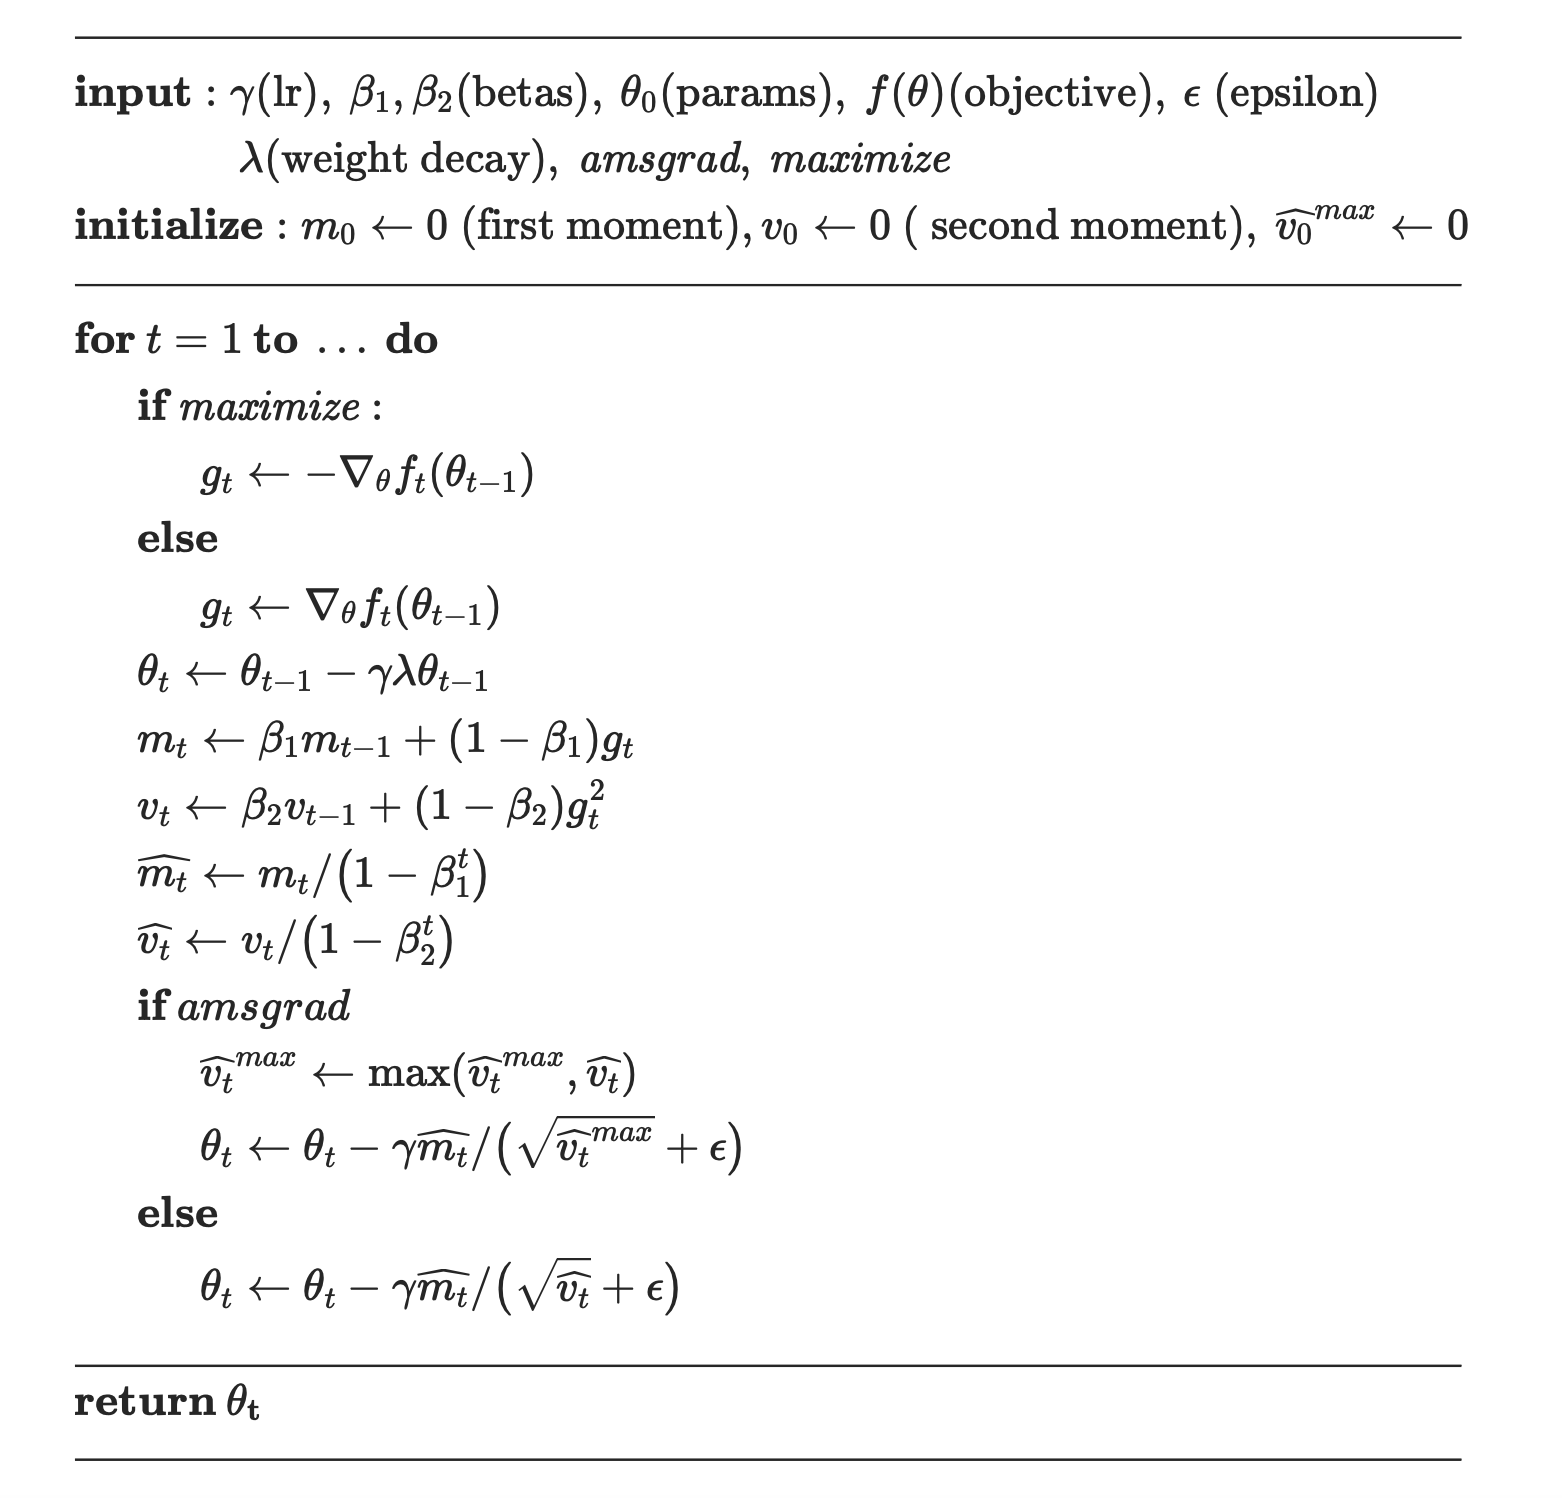
\includegraphics[width=0.7\linewidth]{AdamW.png}
    \caption{Illustration de l'optimiseur AdamW}
    \label{fig:adamw}
\end{figure}

\subsubsection{Fondements mathématiques de l'AdamW}
L'AdamW est une amélioration de l'optimiseur Adam. Il fonctionne en modifiant légèrement la manière dont le modèle est ajusté pendant l'entraînement. Ceci est fait pour rendre le modèle plus stable et performant. Pour obtenir de meilleurs résultats de manière plus efficace, il suit certaines règles spécifiques pour ajuster le modèle :

Sans perte de poids:
\begin{equation}
    \theta_{t+1} = \theta_t - \alpha M_t \nabla f_t(\theta_t)
\end{equation}

Avec perte de poids dans le cas de AdamW:
\begin{equation}
    \theta_{t+1} = (1 - \lambda) \theta_t - \alpha M_t \nabla f_t(\theta_t)
\end{equation}

Ici, $M_t$ intègre des ajustements adaptatifs du taux d'apprentissage, $\alpha$ est le taux d'apprentissage et $(1 - \lambda) \theta_t$ applique la dégradation du poids directement aux poids. \\

À part AdamW, il existe d'autres outils que nous aurions pu utiliser pour ajuster notre modèle, comme SGD (Stochastic Gradient Descent) ou RMSprop. Ces outils aident aussi à améliorer le modèle pendant l'entraînement et ont leurs propres avantages. Cependant, d'après nos lectures, ils ne sont pas toujours les meilleurs pour gérer certains types de données moins fréquentes et ils peuvent nécessiter des ajustements plus précis pour fonctionner correctement. C'est pourquoi nous avons choisi d'utiliser AdamW, qui semble plus adapté.

\subsubsection{Learning rate et epsilon}
Choisir le bon taux d'apprentissage est très important pour améliorer nos modèles. Il y a une grande différence dans les résultats lorsque nous utilisons un certain taux comparé à un autre, surtout pour améliorer des modèles comme BERT. Les études montrent que $2e-5$ fonctionne bien pour diverses tâches dans le domaine du traitement automatique du langage naturel. \cite{devlin2018bert} \\

Ce taux d'apprentissage plus faible est souvent préféré pour les ajustements sensibles de modèles complexes comme BERT et CamemBERT. L'idée est de faire de petits changements précis dans le modèle, ce qui est nécessaire lorsqu'il a déjà été pré-entraîné sur un vaste ensemble de données et qu'il ne lui faut que de légères modifications pour une tâche spécifique. \\

Nous avons aussi choisi d'utiliser la valeur epsilon par défaut ($eps=1e-8$). Cette valeur assure la stabilité du processus d'entraînement, en évitant les divisions par zéro dans l'algorithme d'optimisation. \cite{loshchilov2017decoupled} 

\subsection{Les avantages de Bert et Camembert}
Ces modèles apportent des avancées significatives comparées aux méthodes telles que le word embedding et la modélisation de sujets par LDA. Leur capacité à traiter des données non structurées et à capturer les relations sémantiques subtiles sont essentielles pour identifier correctement les informations pertinentes dans nos données. \\

En somme, ils apportent plusieurs avantages :
\begin{itemize}
    \item Une compréhension du contexte améliorée
    \item Une adaptation linguistique (spécialement conçus pour le français)
    \item Une sélection plus pertinente des articles
\end{itemize}

\subsection{Séparation des données et entrainement du modèle}
Les données sont divisées en ensembles d'entraînement et de test. Les colonnes de texte sont utilisées comme caractéristiques (features), et les labels sont utilisés comme cibles (targets). La fonction train\_test\_split de sklearn.model\_selection est utilisée pour diviser les données, avec un paramètre test\_size définissant la proportion des données à utiliser pour le test. \\

Les données d'entraînement et de test sont préparées pour être compatibles avec le modèle BERT/CamemBERT. Cela implique la tokenisation des textes. Le modèle CamemBERT est entraîné sur les données d'entraînement et évalue ses performances sur l'ensemble de validation.

\subsection{Clustering}
Nous utilisons le clustering dans le but d'identifier les sujets dominants parmis les articles pertinents. Avant d'effectuer le clustering, il est nécessaire de préparer les données.

\subsubsection{Analyse en Composantes Principales (PCA)}
Nous réalisons une analyse en composantes principales qui permet de réduire la dimensionnalité des données pour faciliter le clustering. Pour choisir le nombre de composante, nous utilisons la courbe de la variance expliquée cumulée. La courbe permet d'identifer le point où l'ajout de nouvelles composantes n'apporte plus de gain significatif en variance expliquée. L'ACP est ensuite réalisée en gardant le nombre de composantes nécessaires déterminé grâce à la courbe.

\subsubsection{Choix du nombre de cluster et clustering}
Nous utilisons la méthode du coude pour déterminer le nombre optimal de clusters. Elle implique de faire varier le nombre de clusters (k) et de calculer pour chaque k la somme des carrés des distances entre les points et leur centre de cluster le plus proche. En traçant ces valeurs, on recherche un point où l'ajout de nouveaux clusters n'apporte pas de réduction significative de l'inertie, ce qui indique un bon compromis entre le nombre de clusters et la distance au sein des clusters. \\

Nous utilisons le modèle K-Means avec le nombre optimal de clusters identifié à l'étape précédente. Le modèle assigne chaque point de données à l'un des k clusters en minimisant la distance entre les points de données et le centre de leur cluster respectif. Après l'entraînement, chaque point de données se voit attribuer une étiquette de cluster, indiquant le cluster auquel il appartient.

\subsubsection{Interprétation des cluster}
Les clusters formés peuvent être interprétés de plusieurs manières différentes pour repérer les sujets dominants parmi les articles pertinents. Il est possible d'examiner les mots-clés les plus fréquemment rencontrés dans chaque cluster, ce qui peut révéler les thèmes ou sujets dominants. De plus, en analysant les articles les plus proches des centroïdes de chaque cluster, nous pouvons obtenir des aperçus représentatifs des sujets dominants associées à chaque groupe.

\subsection{Inférence statistique dans le contexte de classification et clustering}
Pour la classification, nous avons calculé les intervalles de confiance pour la précision, le rappel, et le score F1. Ces intervalles de confiance nous permettent de déterminer avec quelle certitude nous pouvons attendre que les performances observées de notre modèle se généralisent à de nouvelles données. 

Pour le clustering, nous avons utilisé l'indice de silhouette pour évaluer la qualité des clusters. Cet indice mesure à quel point chaque point de données est similaire aux autres points dans son propre cluster par rapport aux points dans les clusters voisins. 

Ces approches d'inférence statistique permettent d'assurer que nos modèles fournissent des résultats fiables.

\section{Conclusions}
Notre question de recherche consiste à trouver comment exploiter au mieux les données textuelles qui n'ont pas encore été pleinement utilisées par les gouvernements, en se focalisant sur la sécurité alimentaire en Afrique de l'Ouest.\\

Grâce à nos choix modélisations utilisant CamemBERT, nous pouvons approfondir notre compréhension des dynamiques de la sécurité alimentaire dans cette région. Nos modèles permettent d'améliorer la sélection des articles pertinents en capturant les nuances linguistiques spécifiques. L'application du clustering permet d'identifier et de catégoriser les sujets dominants parmi les articles pertinents. \\

En résumé, nos modélisations contribuent de manière significative à répondre à notre question de recherche grâce à une meilleure compréhension des données textuelles.

\bibliographystyle{unsrt}
\bibliography{references}

\end{document}
